%% DO NOT CHANGE
\documentclass[twoside,9pt,journal,letterpage]{IEEEtran}
\usepackage{cite}
\usepackage{amsmath,amssymb,amsfonts}
\usepackage{algorithmic}
\usepackage{graphicx}
\usepackage{textcomp}
\def\BibTeX{{\rm B\kern-.05em{\sc i\kern-.025em b}\kern-.08em
    T\kern-.1667em\lower.7ex\hbox{E}\kern-.125emX}}
%% DO NOT CHANGE

% Run through MikTeX TexWorks once with auto-install missing packages enabled.

\let\labelindent\relax
\usepackage[shortlabels]{enumitem}
\usepackage{float}
\setlength{\textfloatsep}{5pt}

\usepackage{datetime}
\newdateformat{monthdayyeardate}{%
  \monthname[\THEMONTH]~\THEDAY, \THEYEAR}

\newcommand{\titlestr}{Adaptive Clocking Techniques for SoC Supply Droop Response in Predictive 7nm CMOS}
\title{\titlestr}

\usepackage{lipsum}

%\author{
%\authorblockN{Dan Fritchman}
%\authorblockA{Department of Electrical Engineering and Computer Sciences\\
%University of California, Berkeley\\
%Berkeley, California  94720\\
%Email: dan\_fritchman@berkeley.edu}
%\and
%\authorblockN{Wahid Rahman}
%\authorblockA{Department of Electrical Engineering and Computer Sciences\\
%University of California, Berkeley\\
%Berkeley, California  94720\\
%Email: wahid.rahman@berkeley.edu}
%}

\author{
	Dan Fritchman, \IEEEmembership{Member, IEEE} and Wahid Rahman, \IEEEmembership{Member, IEEE}
	\thanks{Date of publication \monthdayyeardate\today.}
	\thanks{
		D. Fritchman and W. Rahman are with the Department of Electrical Engineering and Computer Sciences, University of California, Berkeley, Berkeley, CA 94720 USA (e-mail: dan\_fritchman@berkeley.edu; wahid.rahman@berkeley.edu).}
	\thanks{
		This work was supported by Professor Borivoje Nikoli\'{c}.}
}

\markboth{UC Berkeley Proceedings of EE241B, March 2020}{Fritchman \MakeLowercase{\textit{and}} Rahman: \titlestr}

\pubid{~\copyright~2020 University of California, Berkeley}

\begin{document}
\maketitle
\IEEEpeerreviewmaketitle

\begin{abstract}
Adaptive clock generation techniques have emerged in recent generations of high-performance SoCs to mitigate timing failure due to supply voltage droops. Resilient techniques vary from analog voltage mixing to digital sensing and clock actuation. This work identifies a taxonomy for adaptive clock generation systems: adaptive clock distribution (ACD) and adaptive PLL-based schemes. Reported realizations in state-of-the-art processor SoCs are reviewed and key performance metrics for comparisons are identified. An evaluation plan is also proposed to  compare such systems in a predictive 7nm CMOS technology.
\end{abstract}

\begin{IEEEkeywords}
Adaptive clocking, adaptive frequency, power efficiency, supply-droop mitigation, supply-voltage droop.
\end{IEEEkeywords}

\maketitle

\section{Introduction}

Power management techniques in modern system-on-chips (SoCs) are critical for energy-efficient processors ranging from data servers to mobile devices. SoC thermal dissipation constraints and energy-saving modes necessitate system-level power management to decrease the power supply or reduce the number of active processing cores. Such techniques exhibit a decrease (i.e. droop) in the SoC supply voltage ($V_{DD}$) due to: the controlled decrease of $V_{DD}$ from a supply regulator or DC-DC converter; and the transient $L \frac{di}{dt}$ supply voltage ripple due to sudden current changes through package inductances when dynamically enabling or disabling on-chip processing cores. To maximize processing throughput, SoCs are designed to operate close to the maximum possible clock frequency ($f_{MAX}$) for the target ($V_{DD}$) with minimal guardbanding. Decreasing $V_{DD}$ reduces the drain currents of CMOS transistors, thereby increasing propagation delays in the critical paths of digital logic. If sufficient timing margin is not available in the design, these critical paths can fail to meet timing and cause unrecoverable errors.

\begin{figure}[h]
	\centering
	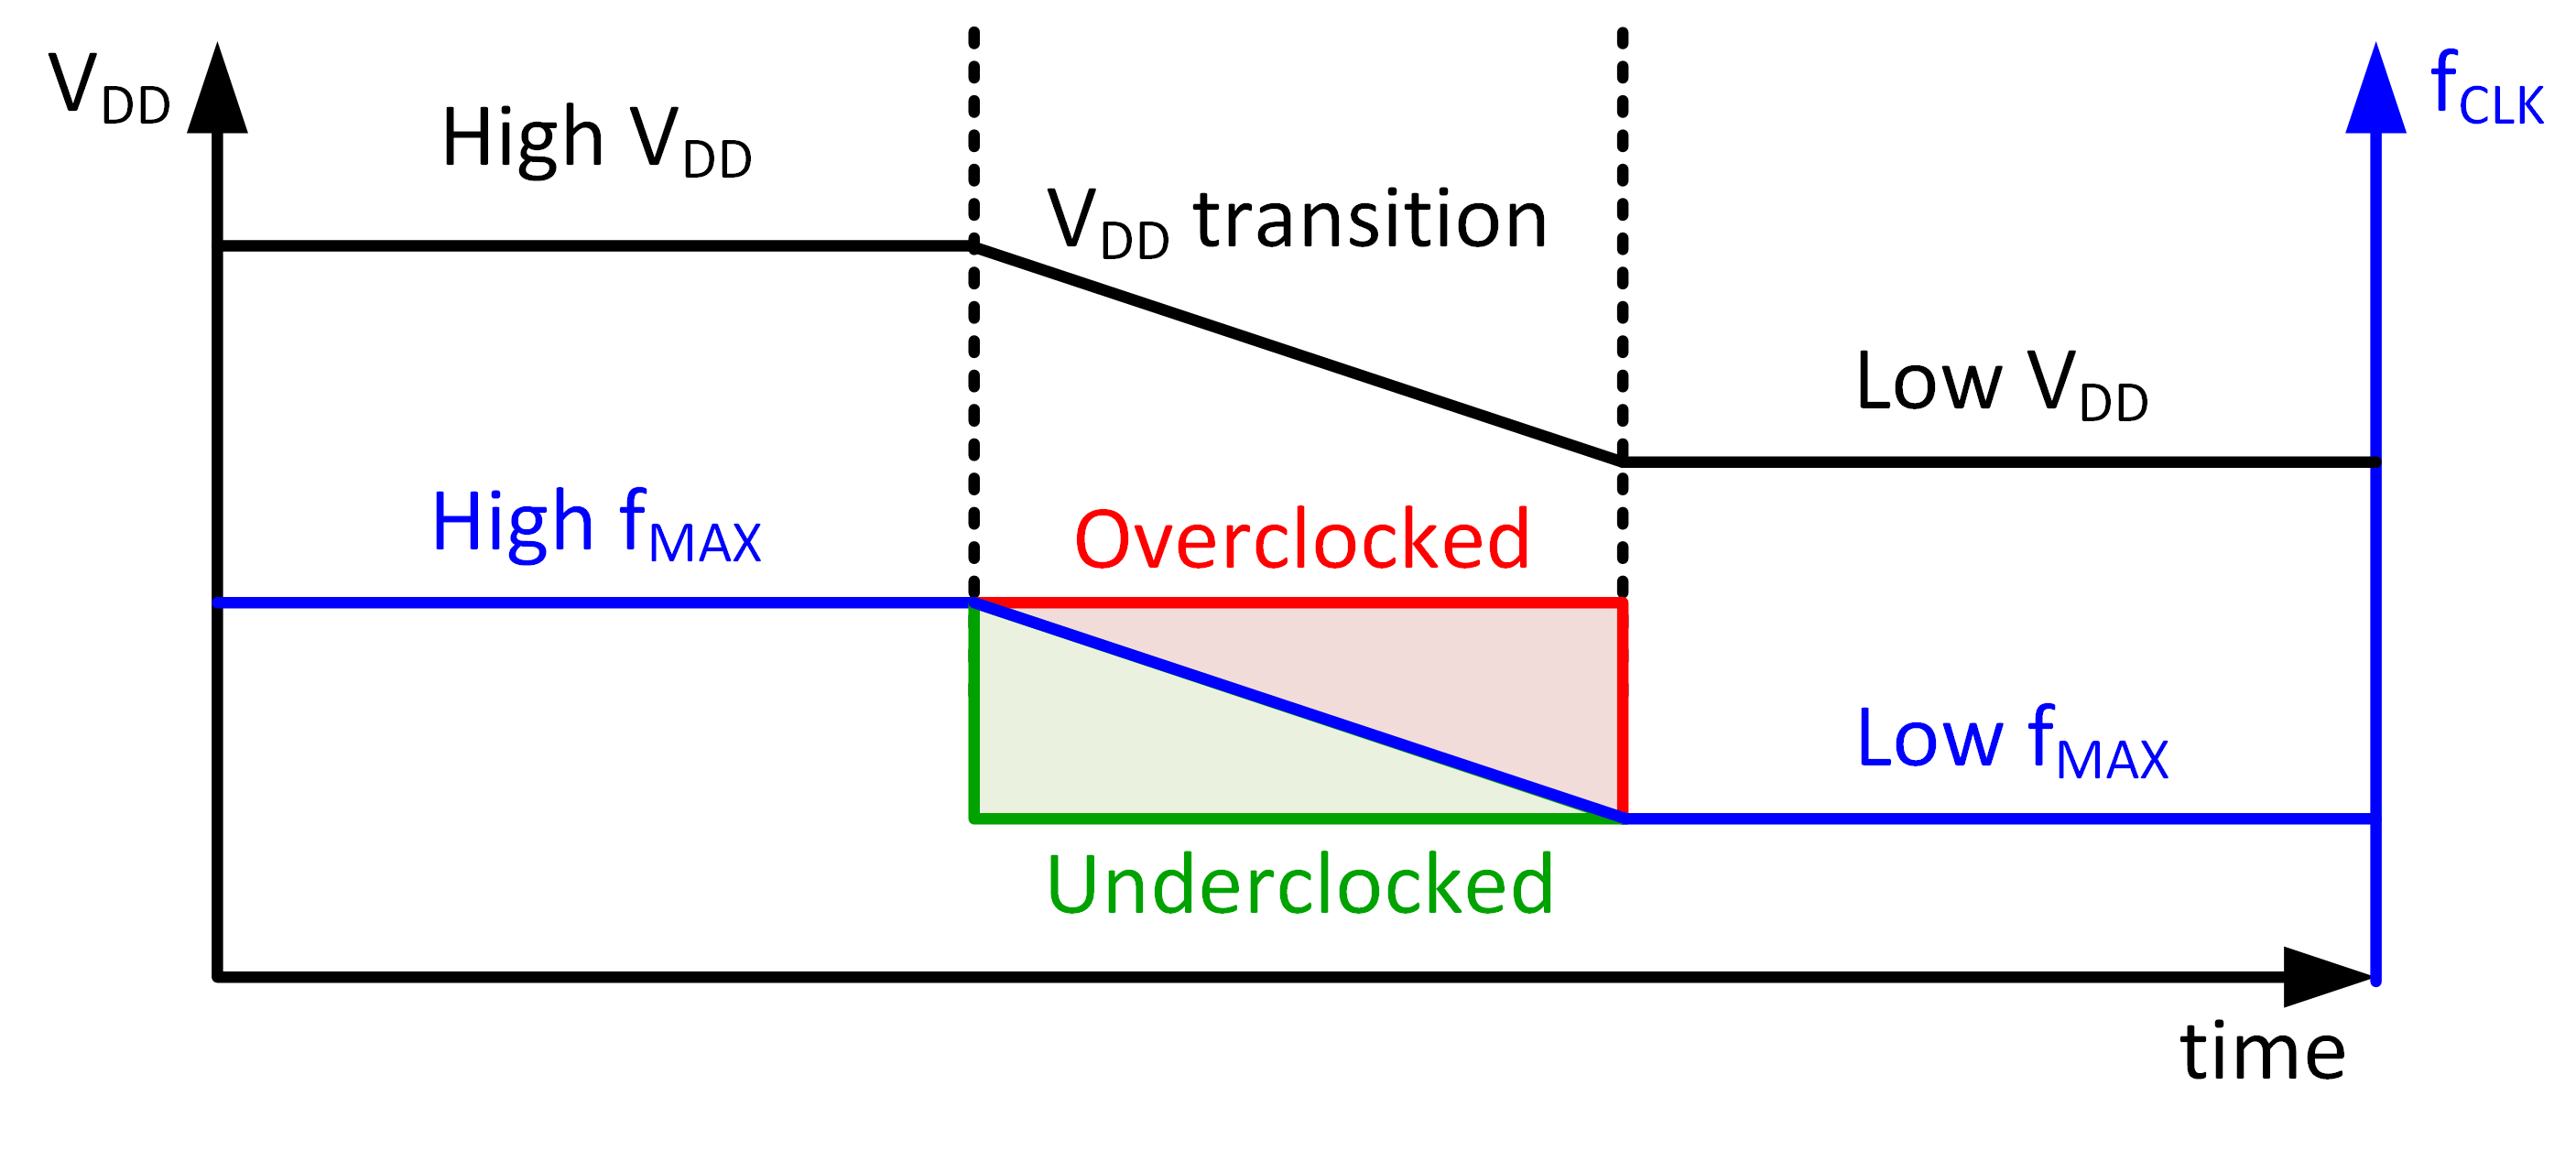
\includegraphics[width=0.85\columnwidth]{fig_fmax}
	\caption{Reduction of $V_{DD}$ and corresponding reduction in $f_{MAX}$ (adapted from \cite{ahmad2017}).}
	\label{fig:fmax}
\end{figure}
\begin{figure}[h]
	\centering
	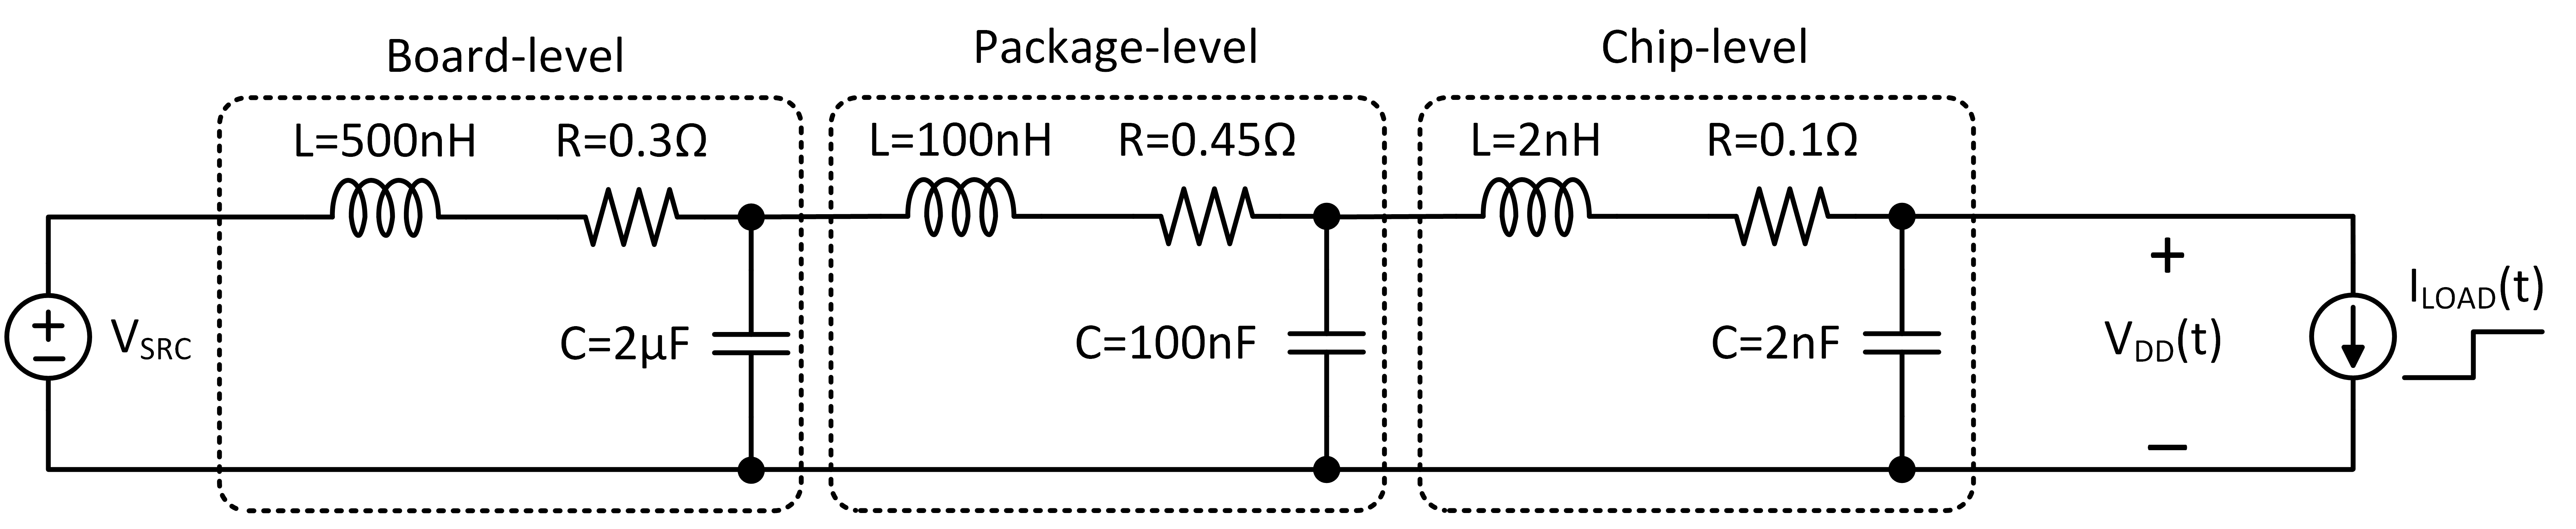
\includegraphics[width=0.85\columnwidth]{fig_droop_schem}
	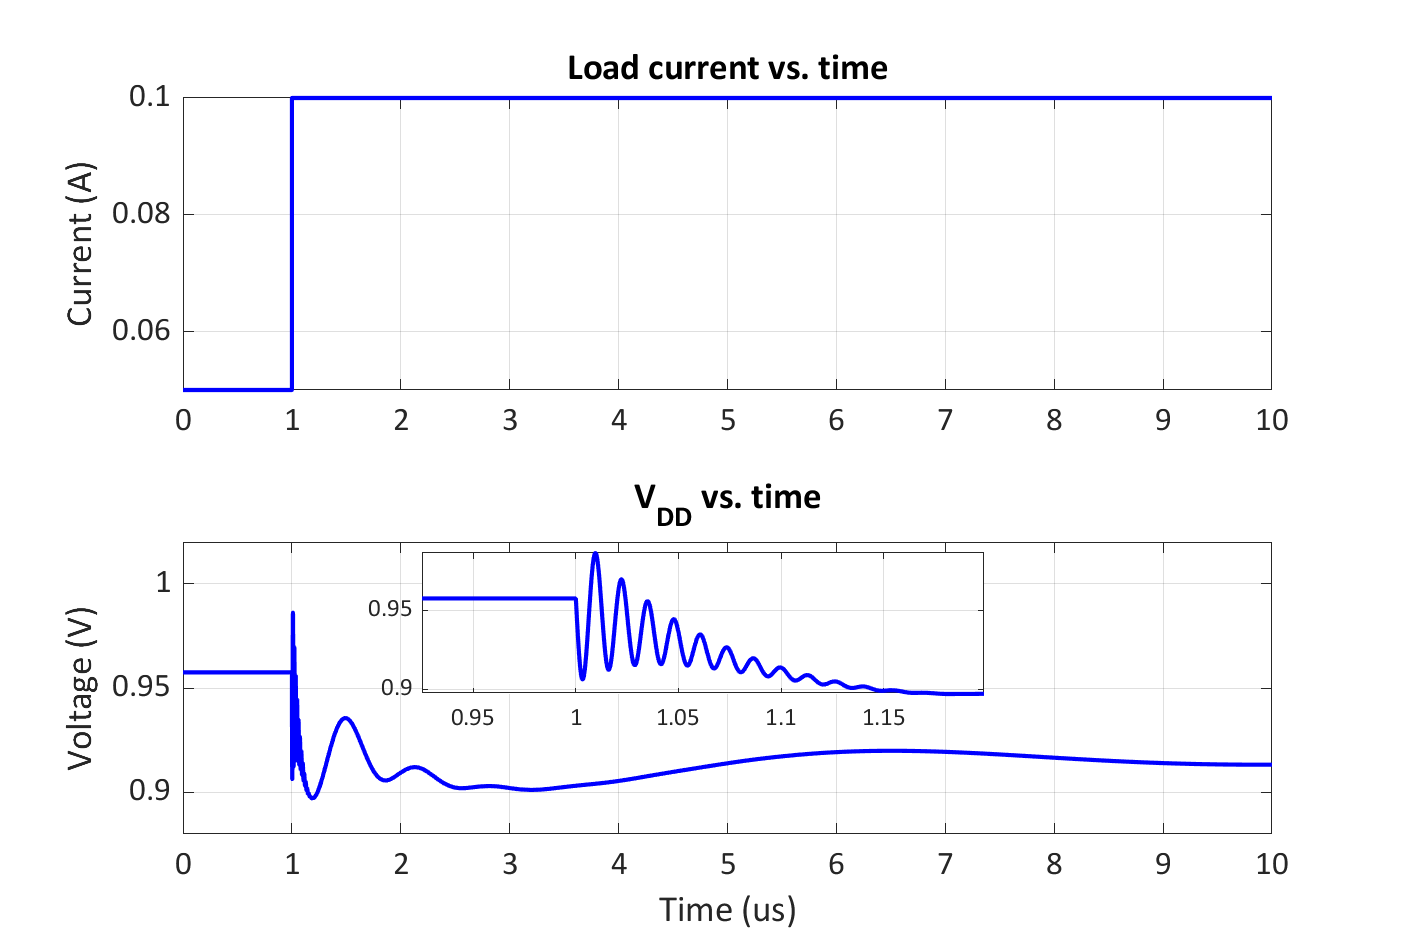
\includegraphics[width=0.85\columnwidth]{fig_droop}
	\caption{Supply droop transients due to package inductances and load current (adapted from \cite{hashimoto2018}).}
	\label{fig:droop}
\end{figure}

To mitigate such failures, adaptive clock generation techniques have emerged in recent generations of high-performance SoCs\cite{ahmad2017,hashimoto2018,wilcox2015,floyd2017,bowman2016}. Adaptive-clock systems detect transient supply events and dynamically adjust clock frequencies to not exceed a changing $f_{MAX}$ as $V_{DD}$ decreases. As Fig.\ \ref{fig:fmax} illustrates, a decrease from high to low $V_{DD}$ to save power corresponds to a decrease in $f_{MAX}$, and the SoC clock frequency ($f_{CLK}$) must track this change without exceeding the correct $f_{MAX}$ (overclocking) and with minimal guardbanding (underclocking) to minimize processing throughput loss during this change\cite{ahmad2017}. 

% If using pudid, place pubidadjcol so it lands in second column of first page
\pubidadjcol
Transient response of adaptive clock techniques is also vital. The external package routes supplying power to the SoC impact supply voltage settling during changes to on-chip core utilization \cite{hashimoto2018}, as illustrated in Fig.\ \ref{fig:droop}. The range of inductances \& capacitances in this network induces a medley of fast and slow time constants. Resilient adaptive clock generation circuits react quickly to fast ripples in $V_{DD}$ ranging from 50-100MHz \cite{hashimoto2018,wilcox2015} while also tracking slower transient settling at 1MHz and below \cite{hashimoto2018,bowman2016,wilcox2015}.




Several schemes exist to realize supply-induced clock adaptation ranging from directly controlling the clock-synthesizing phase-locked loop (PLL)\cite{ahmad2017,hashimoto2018} to modulating a tunable delay line or phase rotator downstream in an adaptive clock distribution (ACD) network\cite{bowman2016,floyd2017,wilcox2015}. In this work, we survey and contrast the adaptive PLL- and ACD-based mechanisms presented in \cite{hashimoto2018} and \cite{wilcox2015}, respectively. This brief is organized as follows: Section \ref{sec:overview} provides an overview of adaptive clocking schemes and defines the scope of this work; Section \ref{sec:details} discusses the operating principles of mechanisms presented in \cite{hashimoto2018} and \cite{wilcox2015}; Section \ref{sec:comparison} provides a comparison of \cite{hashimoto2018} and \cite{wilcox2015}; and finally Section \ref{sec:conclusion} discusses planned work and concludes this brief.

\section{Adaptive Clocking Schemes}
\label{sec:overview}

Adaptive clocking systems include two fundamental components:

\begin{enumerate}[(a)]
\item a \textit{power-supply sensor}, which measures and
reports transient droops in supply voltage; and
\item a \textit{clock period actuator}, which modulates the
system clock period in response to reports from
the power-supply sensor.
\end{enumerate}

During a supply drop, low-latency sensing and actuation is crucial to detect and adjust the clock frequency quickly to ensure error-free operation continues throughout the event. If and when $V_{DD}$ recovers from this event to its nominal value, additional circuitry can assist with managing the corresponding $f_{CLK}$ recovery.

ACD- and adaptive PLL-based systems differ in their implementation of the clock period actuator. ACD-based systems decrease the clock frequency by extending clock periods using an ACD circuit placed between the clock-synthesizing PLL and the global clock distribution network as illustrated in Fig.\ \ref{fig:overview_acd}. A digital code $CTRL_{FCLK}$ from the power supply sensor controls the ACD circuit such that it extends the period of the synthesized clock, $CLK_{PLL}$, to the desired frequency given the sensed change in $V_{DD}$. This lower-frequency clock, $CLK_{SOC}$, is then distributed through the global clock network to the SoC processing cores. Examples of this ACD circuit include tunable-length delay \cite{bowman2016} and phase rotators \cite{wilcox2015}, of which the latter is discussed in Section \ref{sec:details_acd}.

\begin{figure}[h]
	\centering
	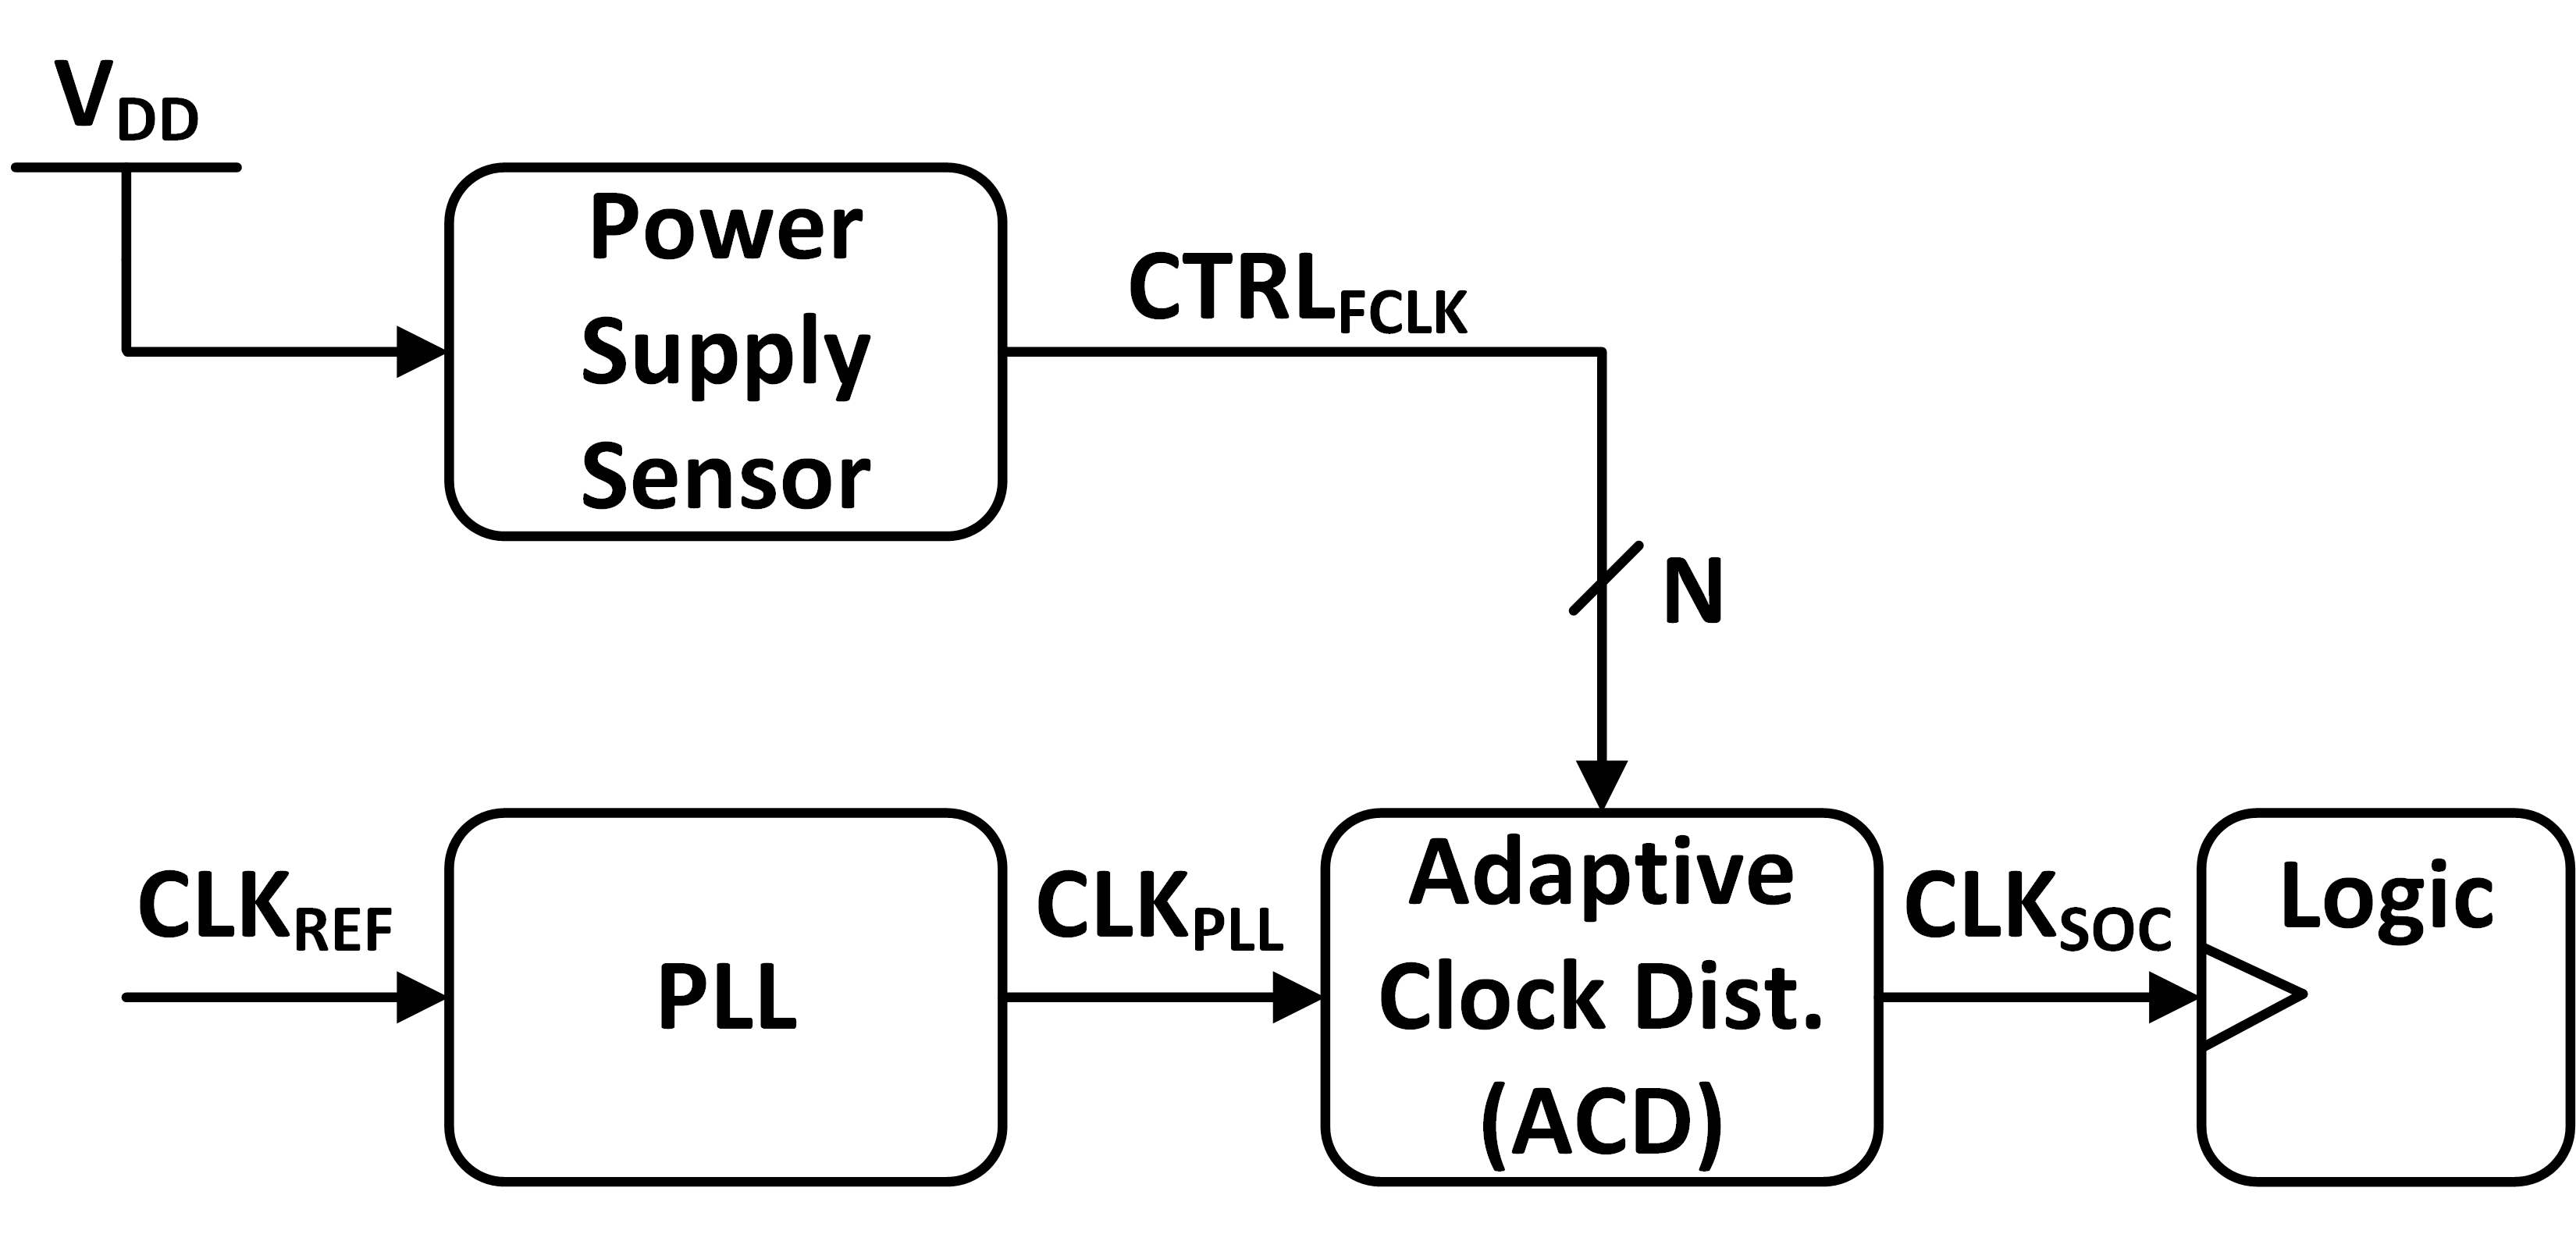
\includegraphics[width=0.7\columnwidth]{fig_overview_acd}
	\caption{Adaptive clock distribution (ACD) based system.}
	\label{fig:overview_acd}
\end{figure}

\begin{figure}[h]
	\centering
	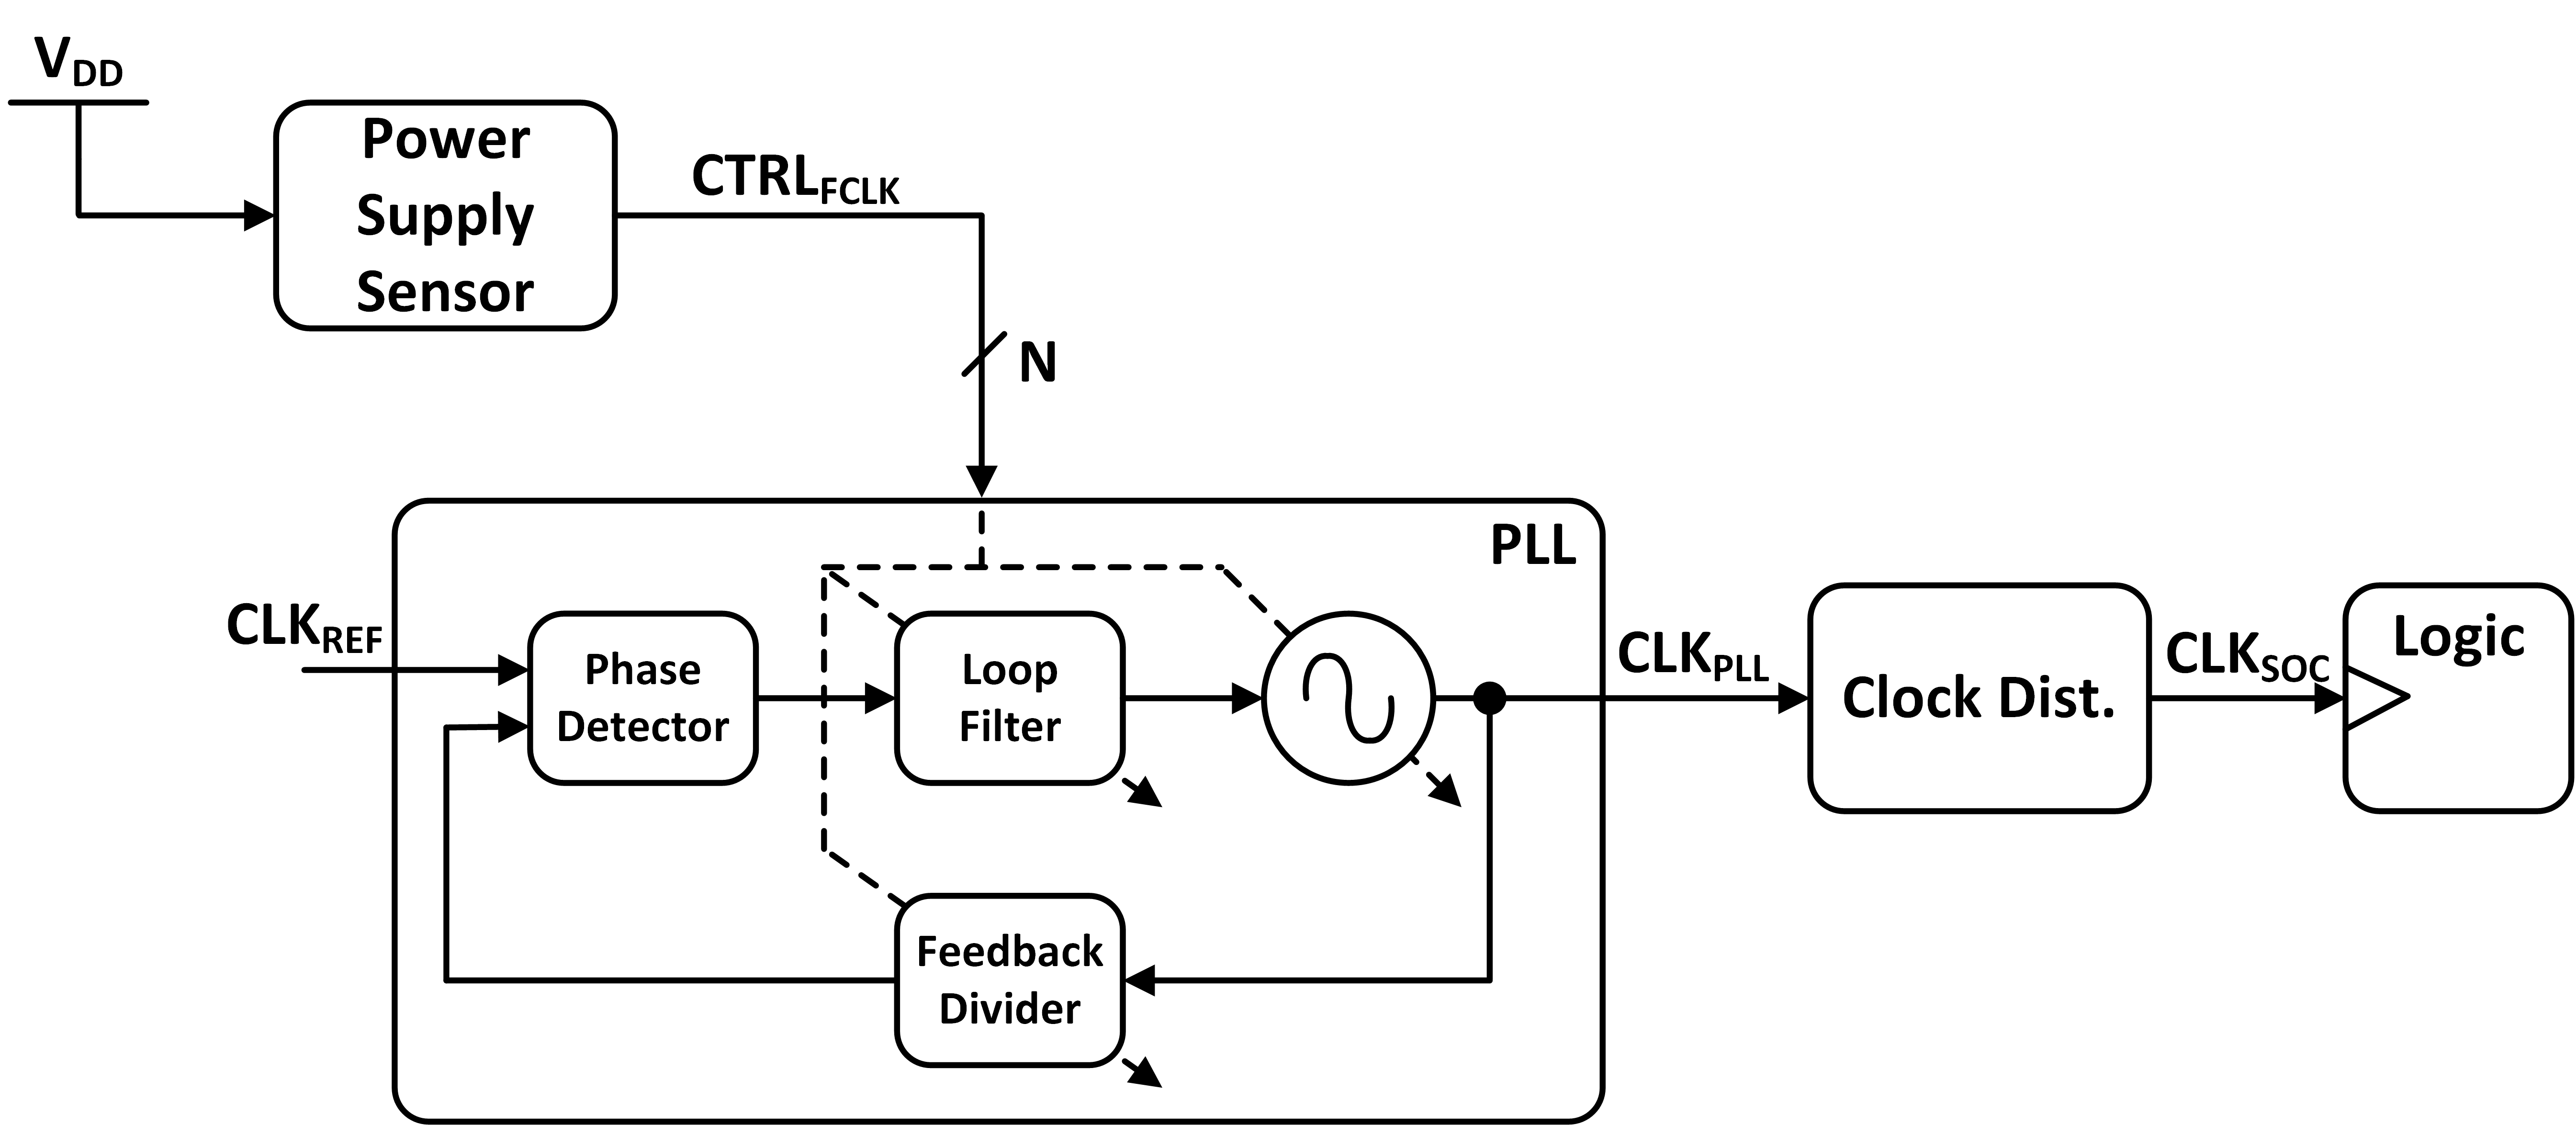
\includegraphics[width=\columnwidth]{fig_overview_pll}
	\caption{Adaptive PLL-based system with possible intra-PLL control variants.}
	\label{fig:overview_pll}
\end{figure}

Adaptive PLL-based systems, in contrast, incorporate information from the power-supply sensor to dynamically change the behaviour of PLL sub-components. Typically, these schemes affect oscillator control on top of the traditional PLL loop. In \cite{ahmad2017} for example, the oscillator is controlled indirectly through a loop filter modified for droop response: when a droop is detected, the traditional proportional- and integral-loop filter switches to proportional-only to form a type-I PLL that tunes the oscillator to frequency lock without hazardous over- or underclocking. In \cite{hashimoto2018}, this idea is further extended by interrupting the PLL feedback loop to modify the oscillator directly, reacting to a supply droop event with relatively low latency. The feedback divider is then slowly modified to restore PLL lock. This latter work is further discussed in Section \ref{sec:details_pll}.

The focus of this brief is to compare the design and effectiveness of clock period actuators in ACD and PLL-based schemes. While high-resolution power-supply sensors and their low-latency integration are critical to the overall adaptation time of such schemes, it remains beyond the scope of this work.

\section{Operating principles}
\label{sec:details}
The two main works for comparison are the PLL- and ACD-based adaptive clocking schemes in \cite{hashimoto2018} and \cite{wilcox2015} respectively. The operating principles of each are described in this section.

\subsection{PLL-based adaptive clocking}
\label{sec:details_pll}
The scheme reported in \cite{hashimoto2018} presents a PLL-based adaptive clocking control for three SPARC processor cores in a 20nm CMOS testchip. A sense point placed near one of the SPARC cores transmits the core $V_{DD}$ through low-impedance on-package (off-chip) routing to the on-chip power-supply sensor. This sensor converts $V_{DD}$ droops into a thermometer-coded quantized digital signal, $q[n]$, by use two calibrated delay lines and a 8-bit time-to-digital converter (TDC). 

A major contribution of \cite{hashimoto2018} is to use the instantaneous value of q[n] to immediately reduce the PLL's oscillator frequency to correct for high-frequency droops and use a filtered version of $q[n]$ to correct for low frequency droops and ultimately re-lock the PLL feedback loop. As shown in Fig.\ \ref{fig:detail_pll} and Fig.\ \ref{fig:detail_pllarch}, $q[n]$ is processed by the frequency control logic to generate two control signals: $\Delta F_{code}$ that can instantaneously respond to changes in $q[n]$ to directly change the digitally-controlled oscillator (DCO) frequency, and $N^{sync}_{code}$ that relies only on a filtered value of $q[n]$ to track low-frequency droops and re-lock the PLL loop at the new frequency by changing the feedback division value. The minimum function and the non-linear filter together effectively construct an all-pass filter when $V_{DD}$ decreases and a low-pass filter when $V_{DD}$ increases. They allow the loop to actuate the clock with minimal latency during a $V_{DD}$ droop event. During droop recovery, they low-pass filter $V_{DD}$ transients and overshoots as the voltage ultimately settles to its nominal value.

\begin{figure}[h]
	\centering
	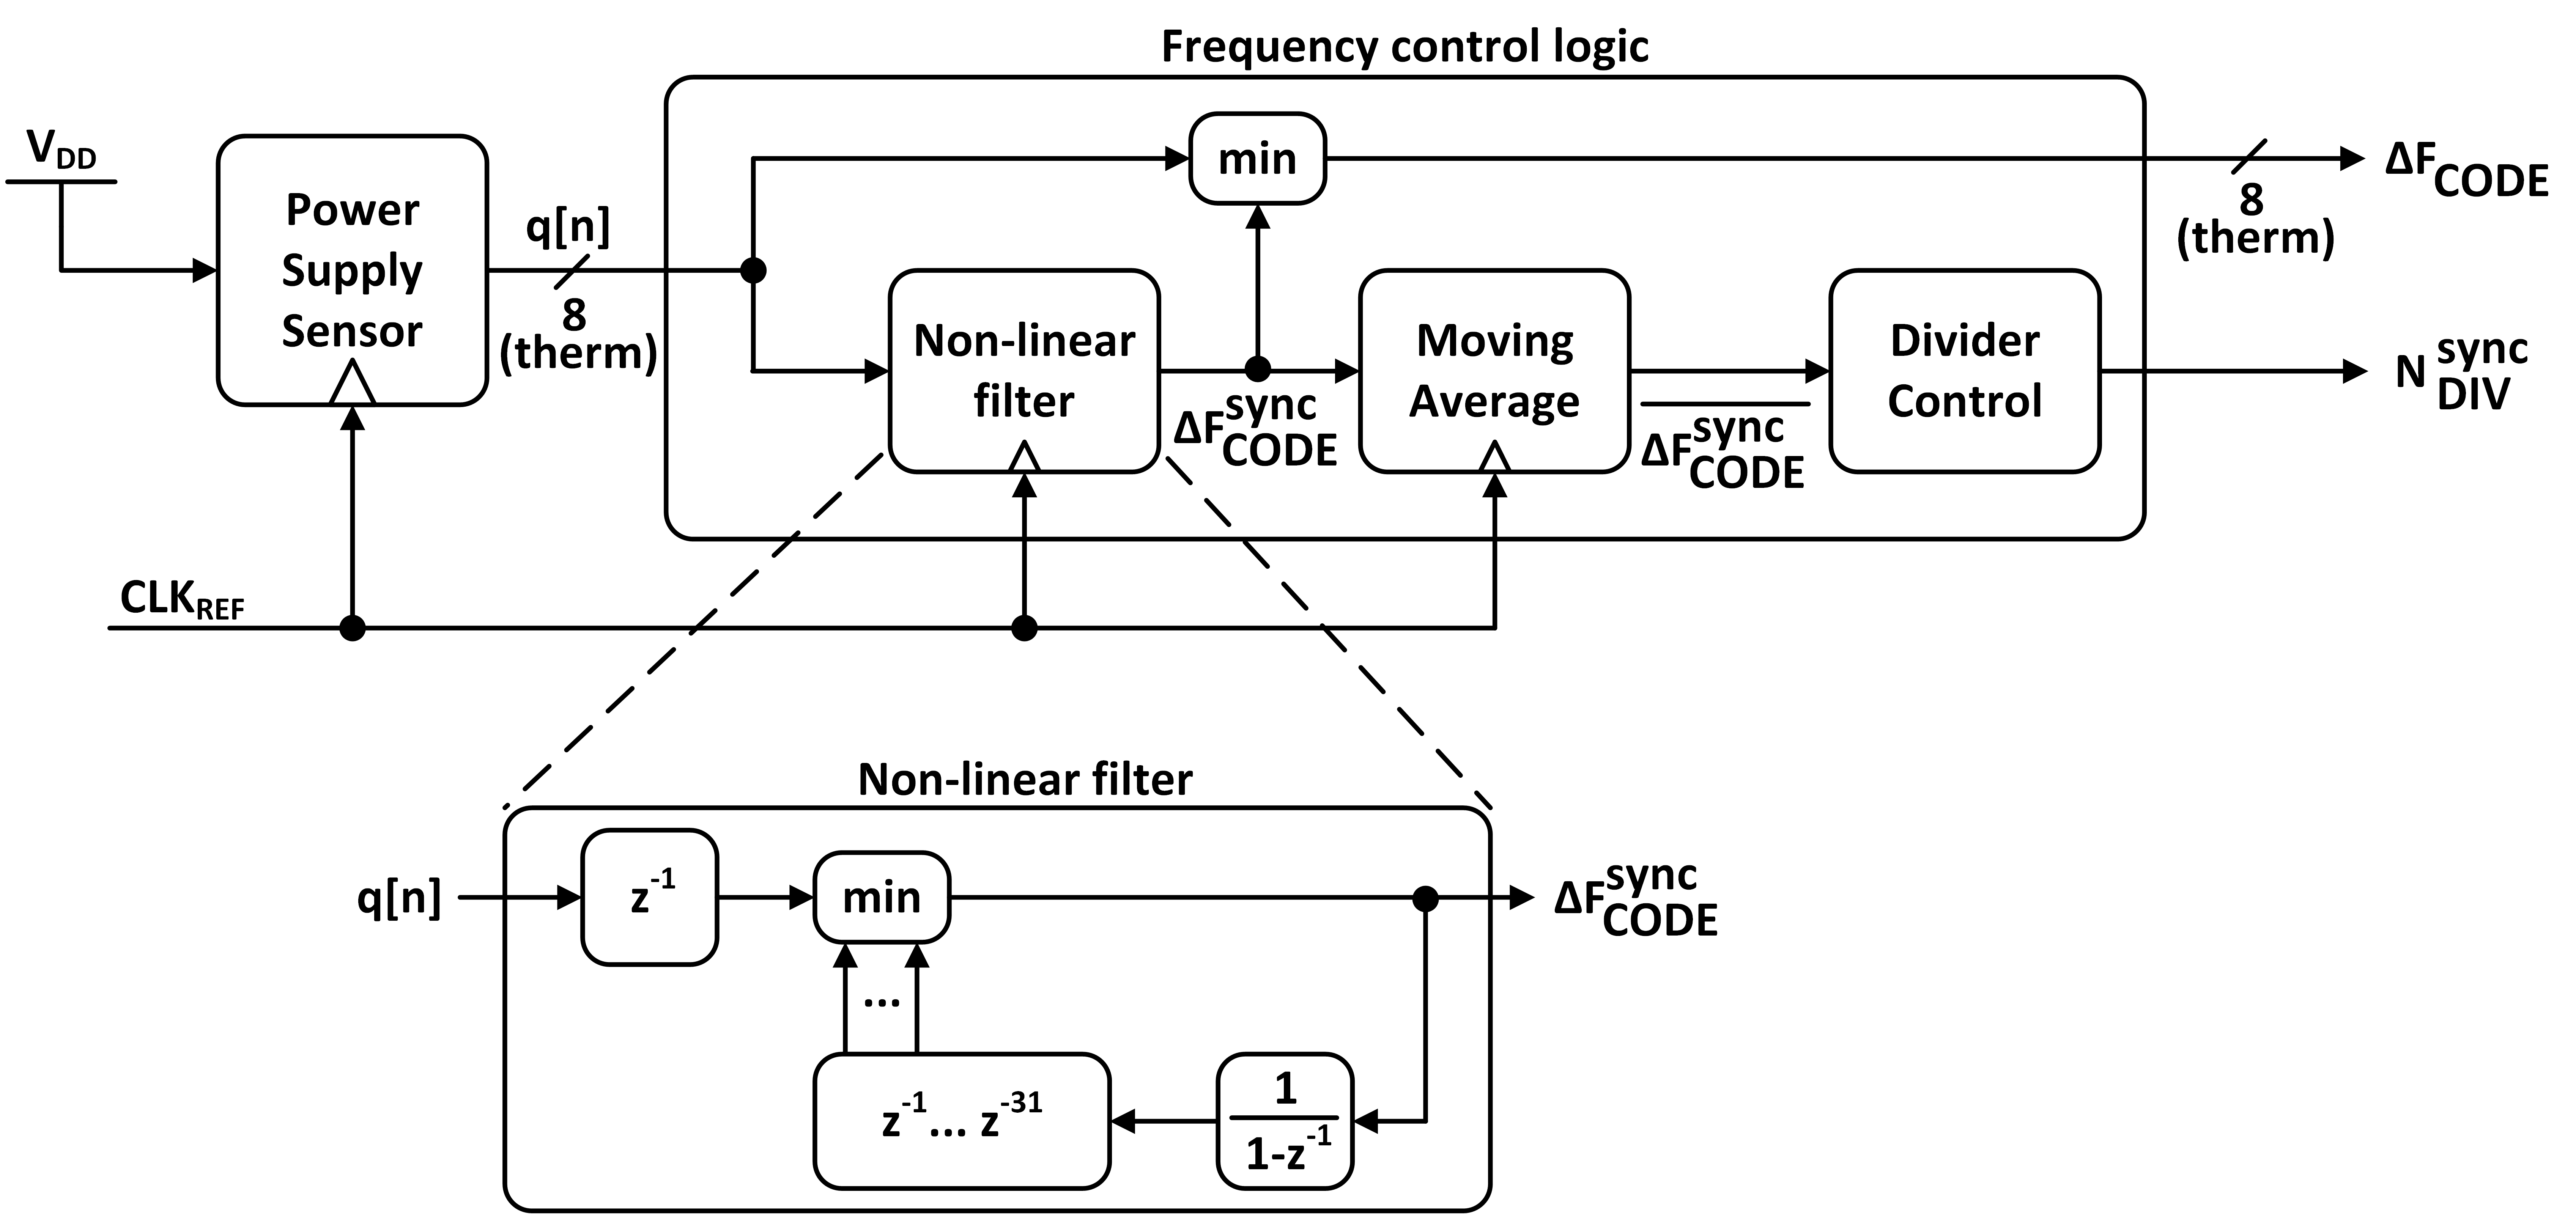
\includegraphics[width=\columnwidth]{fig_detail_pll}
	\caption{Frequency control logic for PLL-based adaptive clocking in \cite{hashimoto2018}.}
	\label{fig:detail_pll}
\end{figure}

\begin{figure}[h]
	\centering
	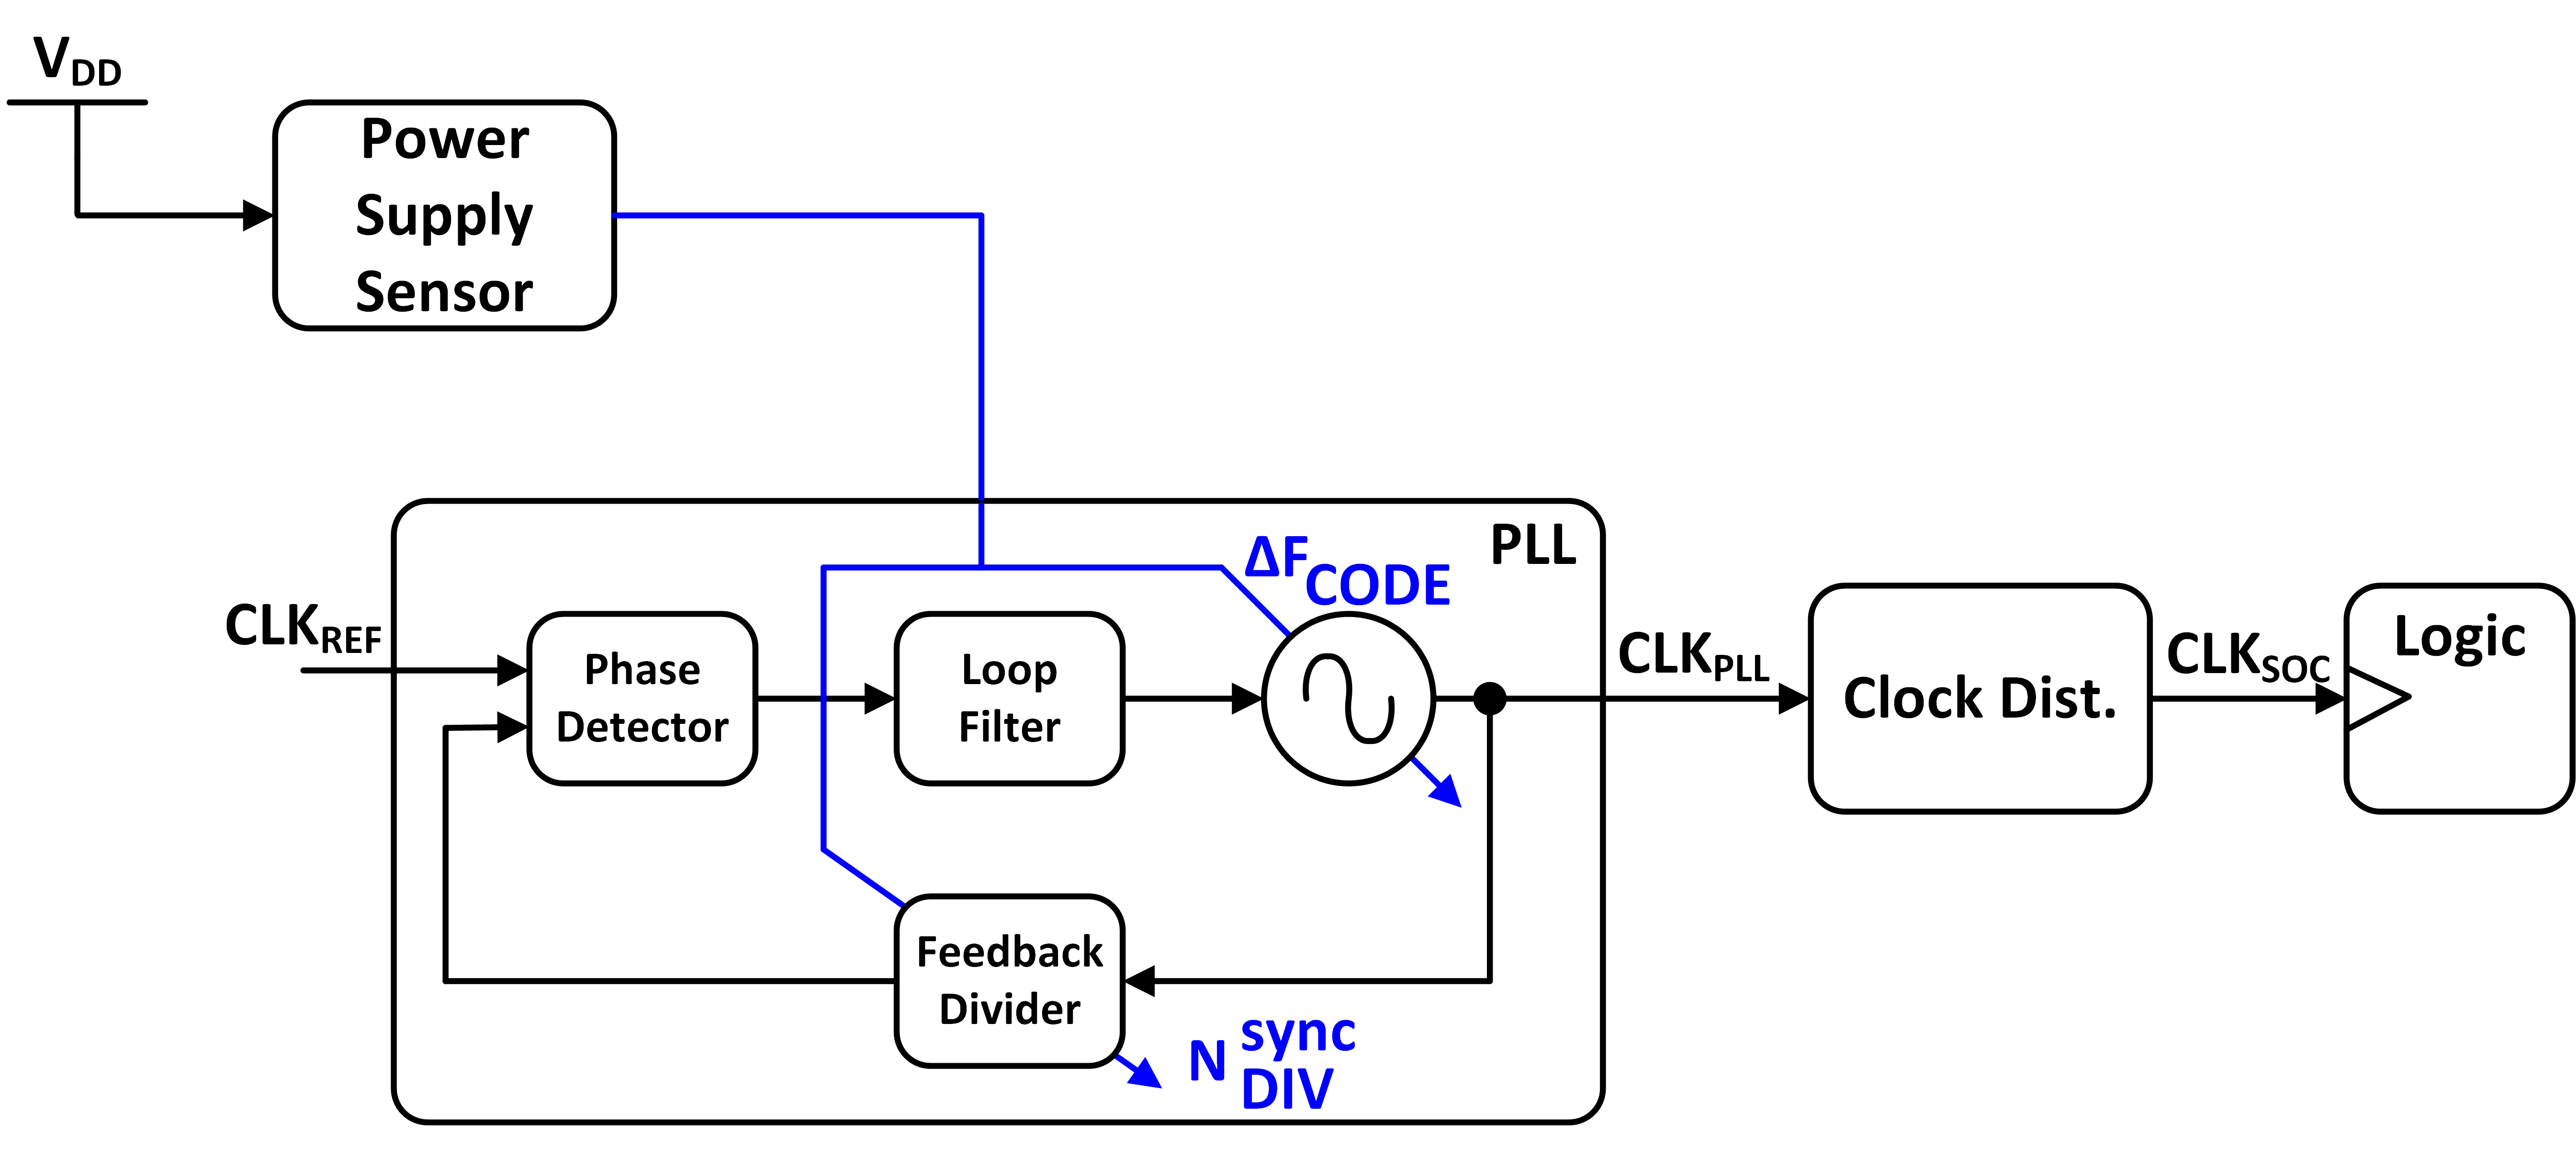
\includegraphics[width=\columnwidth]{fig_detail_pllarch}
	\caption{Intra-PLL control for PLL-based adaptive clocking in \cite{hashimoto2018}.}
	\label{fig:detail_pllarch}
\end{figure}

A fast response to high-frequency supply droops is an important criterion in \cite{hashimoto2018}, significant design efforts were made to ensure low-latency clock period actuation. The reported design target is 8$\times$ faster than the first-droop frequency of 50MHz. This permits a time window of 2.5ns from the time $V_{DD}$ crosses the first supply sensor threshold to the time the SoC clock frequency is corrected. This narrow timing constraint is met by generating and propagating the critical oscillator control signal $\Delta F_{code}$ asynchronously. Crucially, the 8-bit thermometer-coded $\Delta F_{code}$ controls a DCO that can tolerate asynchronous changes in its code without glitching its output clock. The DCO reported in \cite{hashimoto2018} is a bank of nine ring inverters with eight of the rings independently enabled by each thermometer bit of $\Delta F_{code}$. Such a structure can tolerate asynchronous arrival of $\Delta F_{code}$ when suddenly decreasing frequency, as the case of a droop. Note that frequency increases are restricted: the combination of non-linear filter memory with the masking of minimum function ensures $\Delta F_{code}$ only increases one bit at a time after droop recovery \cite{hashimoto2018}. This obviates synchronization of $\Delta F_{code}$, reducing adaptation latency.

The reduction in adaptation latency directly correlates with reported experimental results. Fast response to droops allows for tighter guardbanding and therefore higher $f_{MAX}$. While \cite{hashimoto2018} does not report the exact clock adaptation latency, the work improves $f_{MAX}$ by 7.5\%, from 4.65GHz without adaptive clocking to 5.00GHz with the proposed scheme. This is the largest frequency gain reported in compared works.

\subsection{ACD-based adaptive clocking}
\label{sec:details_acd}
The scheme reported in \cite{wilcox2015} presents a ACD-based adaptive clocking control for AMD's Steamroller CPU in 28nm CMOS. The power supply sensor consists of a DLL-based droop detector acting as a delay line connected to the SoC core $V_{DD}$: as $V_{DD}$ changes, the DLL phases change with respect to a regulated PLL's output clock. A programmable threshold selects one of four DLL phases to compare against the reference PLL phase to signal a 1-bit droop activity.

Fig.\ \ref{fig:detail_acd} illustrates the reported scheme. A DLL-based phase rotator realizes the ACD circuit. When a droop activity is detected and $DroopDetected$ is asserted, phase rotation between the 40 DLL phases occurs to effectively ``stretch" the clock period and reduce the clock frequency. To ensure glitchless phase rotation, small positive pre-programmed phase increments occur at each step, and the phase rotator rotates through all 40 phases before continuing the cycle. Rotation can be bypassed entirely by de-asserting $DroopEnable$. 

\begin{figure}[h]
	\centering
	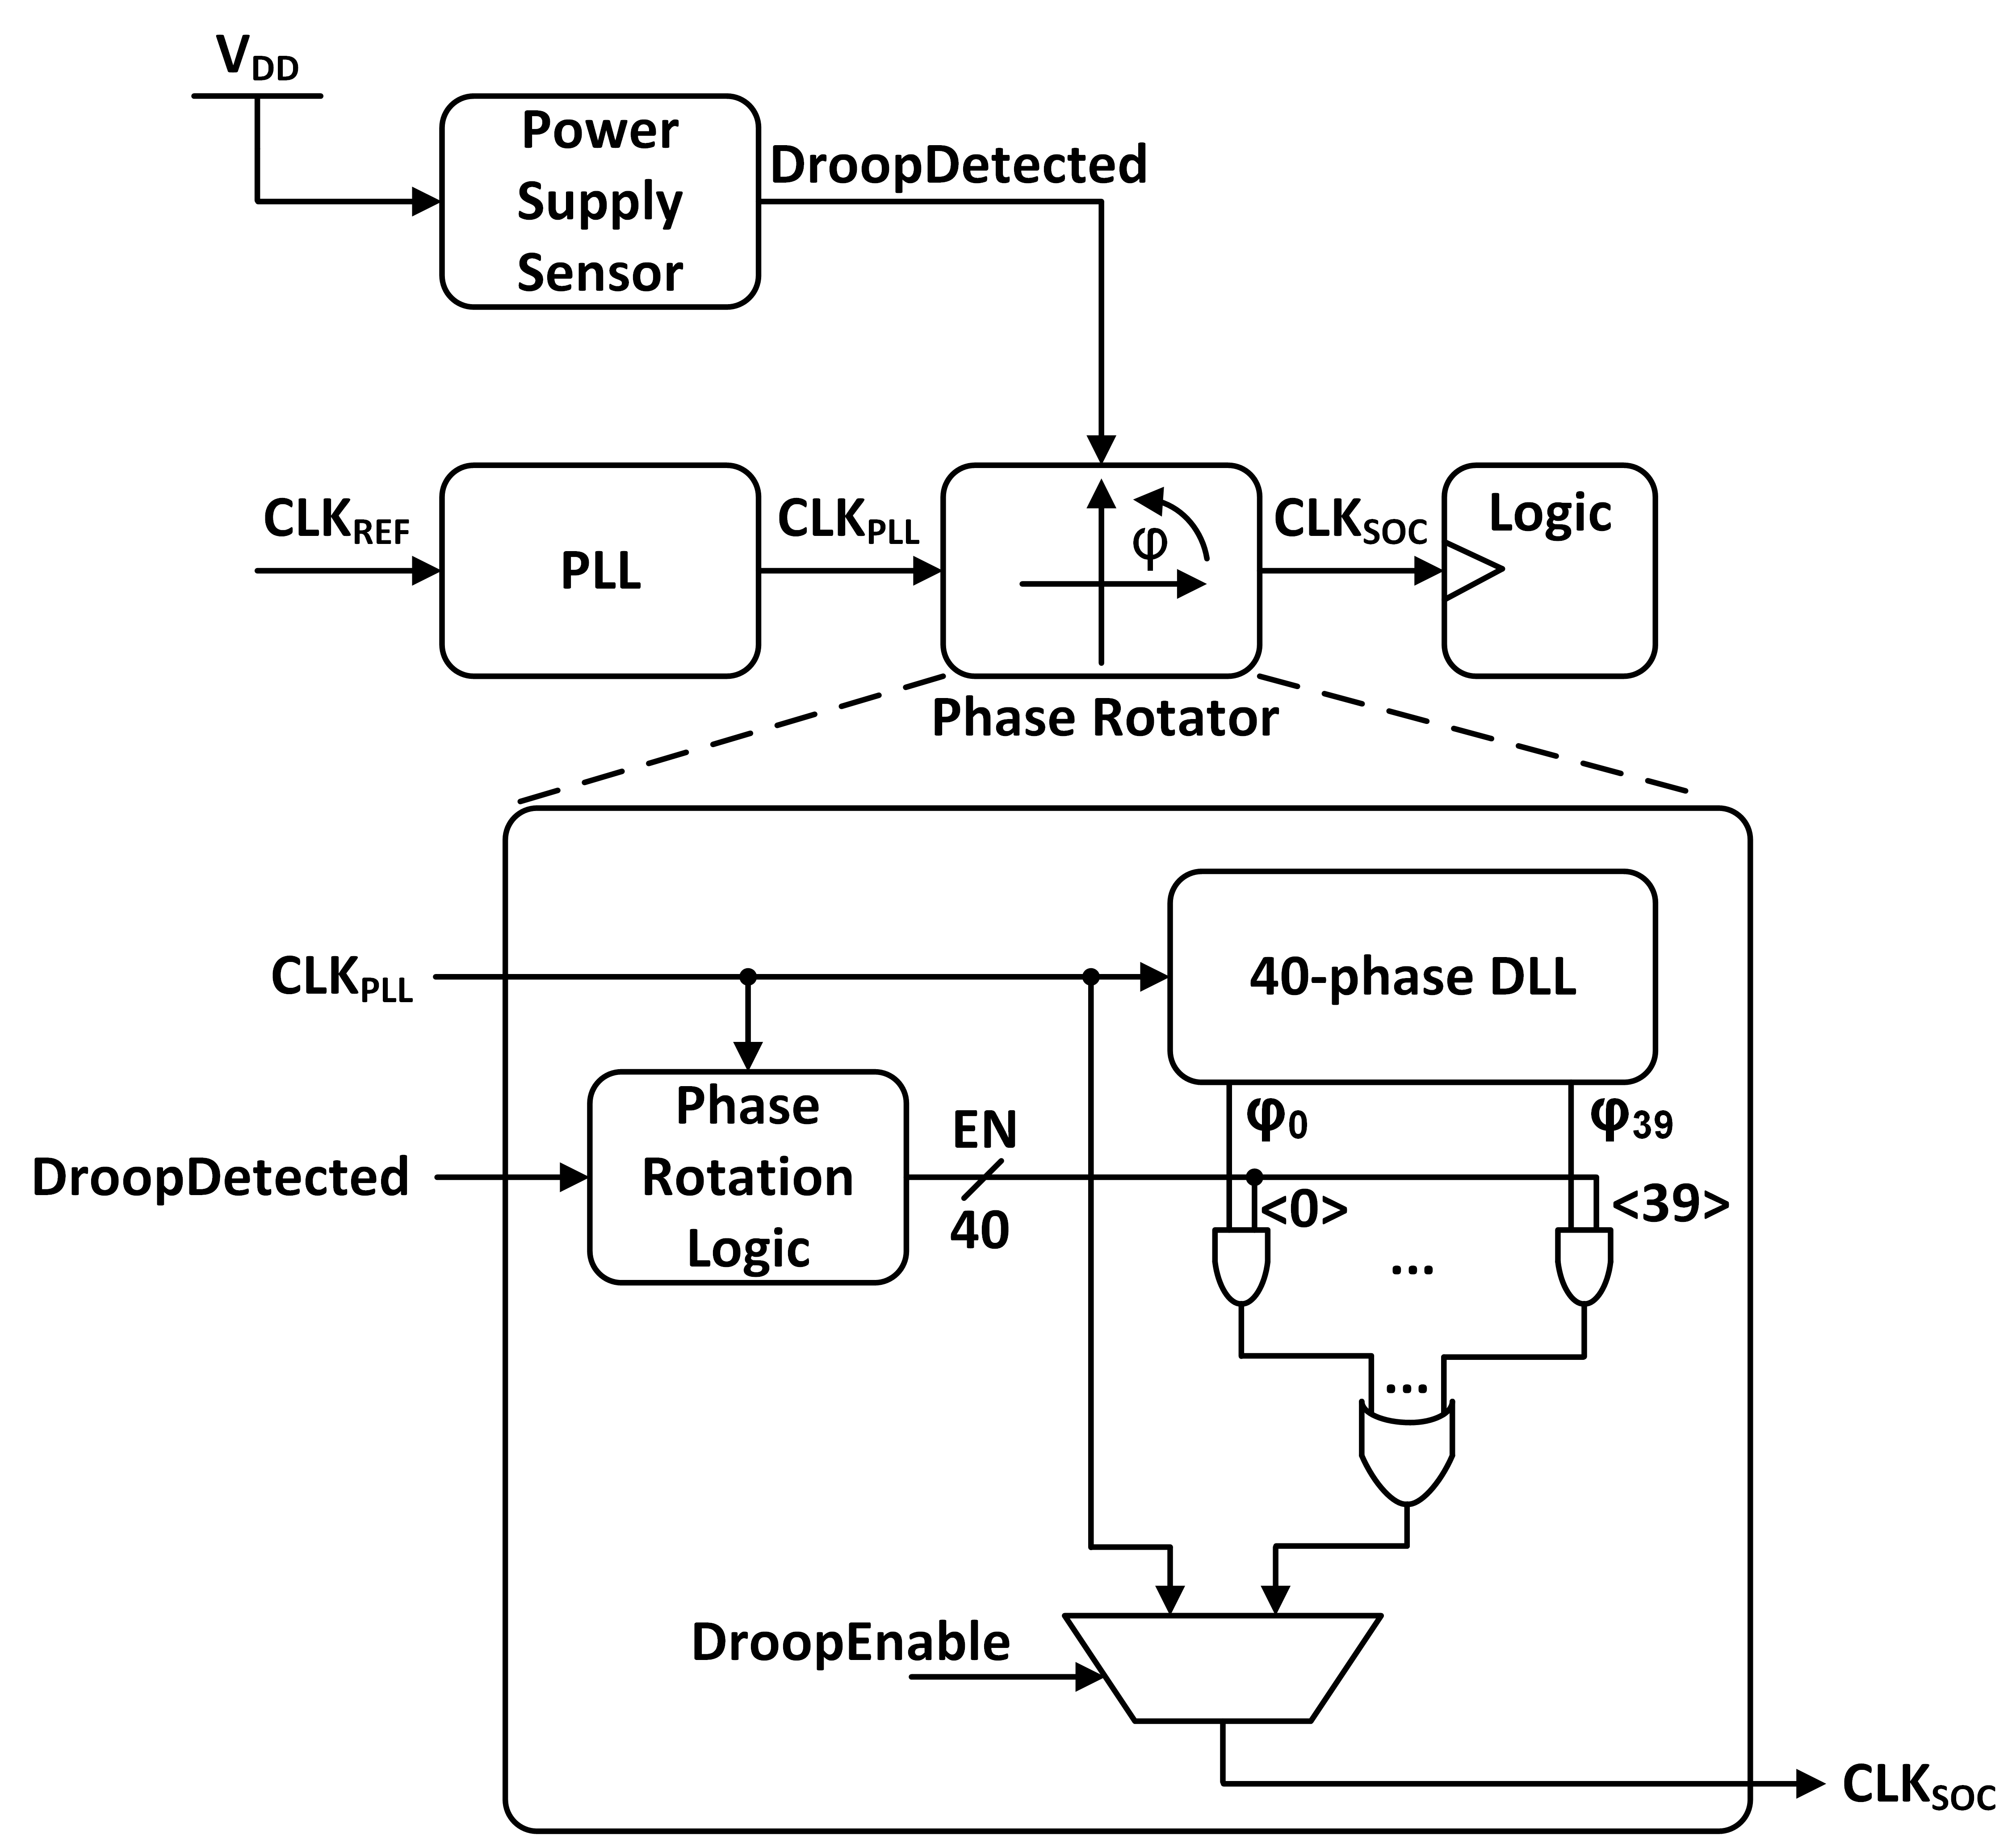
\includegraphics[width=0.7\columnwidth]{fig_detail_acd}
	\caption{Frequency control logic for ACD-based adaptive clocking in \cite{wilcox2015}.}
	\label{fig:detail_acd}
\end{figure}

This scheme reports to target fast initial droops of 100MHz and slower 1-5MHz secondary droop transients by means of the programmed droop detector threshold \cite{wilcox2015}. As the detector signal is binary, the ACD-based reduces the SoC clock frequency by a fixed amount (phase rotator steps through a fixed phase step per cycle) or does not change the frequency at all. Voltage recovery is triggered when $V_{DD}$ crosses back beyond the detector threshold. The work reports a total adaptation latency of 3 cycles at 3.4GHz from droop detection to clock frequency reduction. While experimental results do not report frequency gain as in \cite{hashimoto2018}, silicon results demonstrated a reduction of 3-6\% in $V_{MIN}$, the minimum supply voltage tolerable at a given frequency for the SoC. No comparison was provided with prior works.

\section{Comparison of ACD and PLL Actuators}
\label{sec:comparison}

\subsection{Comparison Scope}
\label{sec:Scope of comparison}

As discussed in Section \ref{sec:overview}, clock adaptation consist of various sub-components and their latencies. This is illustrated in Fig.\ \ref{fig:scope}. Design of a complete adaptation system requires a $V_{DD}$ sense point, routing delay, detector and actuation latencies, and finally clock propagation delay. This comparison focuses on the detection logic, clock actuation, and their combined actuation latency. There are indeed important specifications beyond this when designing adaptation circuits. For example, sensor resolution, bandwidth, and ease of design integration with digital SoCs are important considerations: highly digital sensors \cite{hashimoto2018,wilcox2015} to custom analog voltage mixing \cite{kurd2009} have their bandwidth and integration tradeoffs. However, the scope of this comparison focuses on PLL- and ACD-based adaptive clocking presented in \cite{hashimoto2018} and \cite{wilcox2015} respectively, agnostic to extraneous design considerations.

\begin{figure}[h]
	\centering
	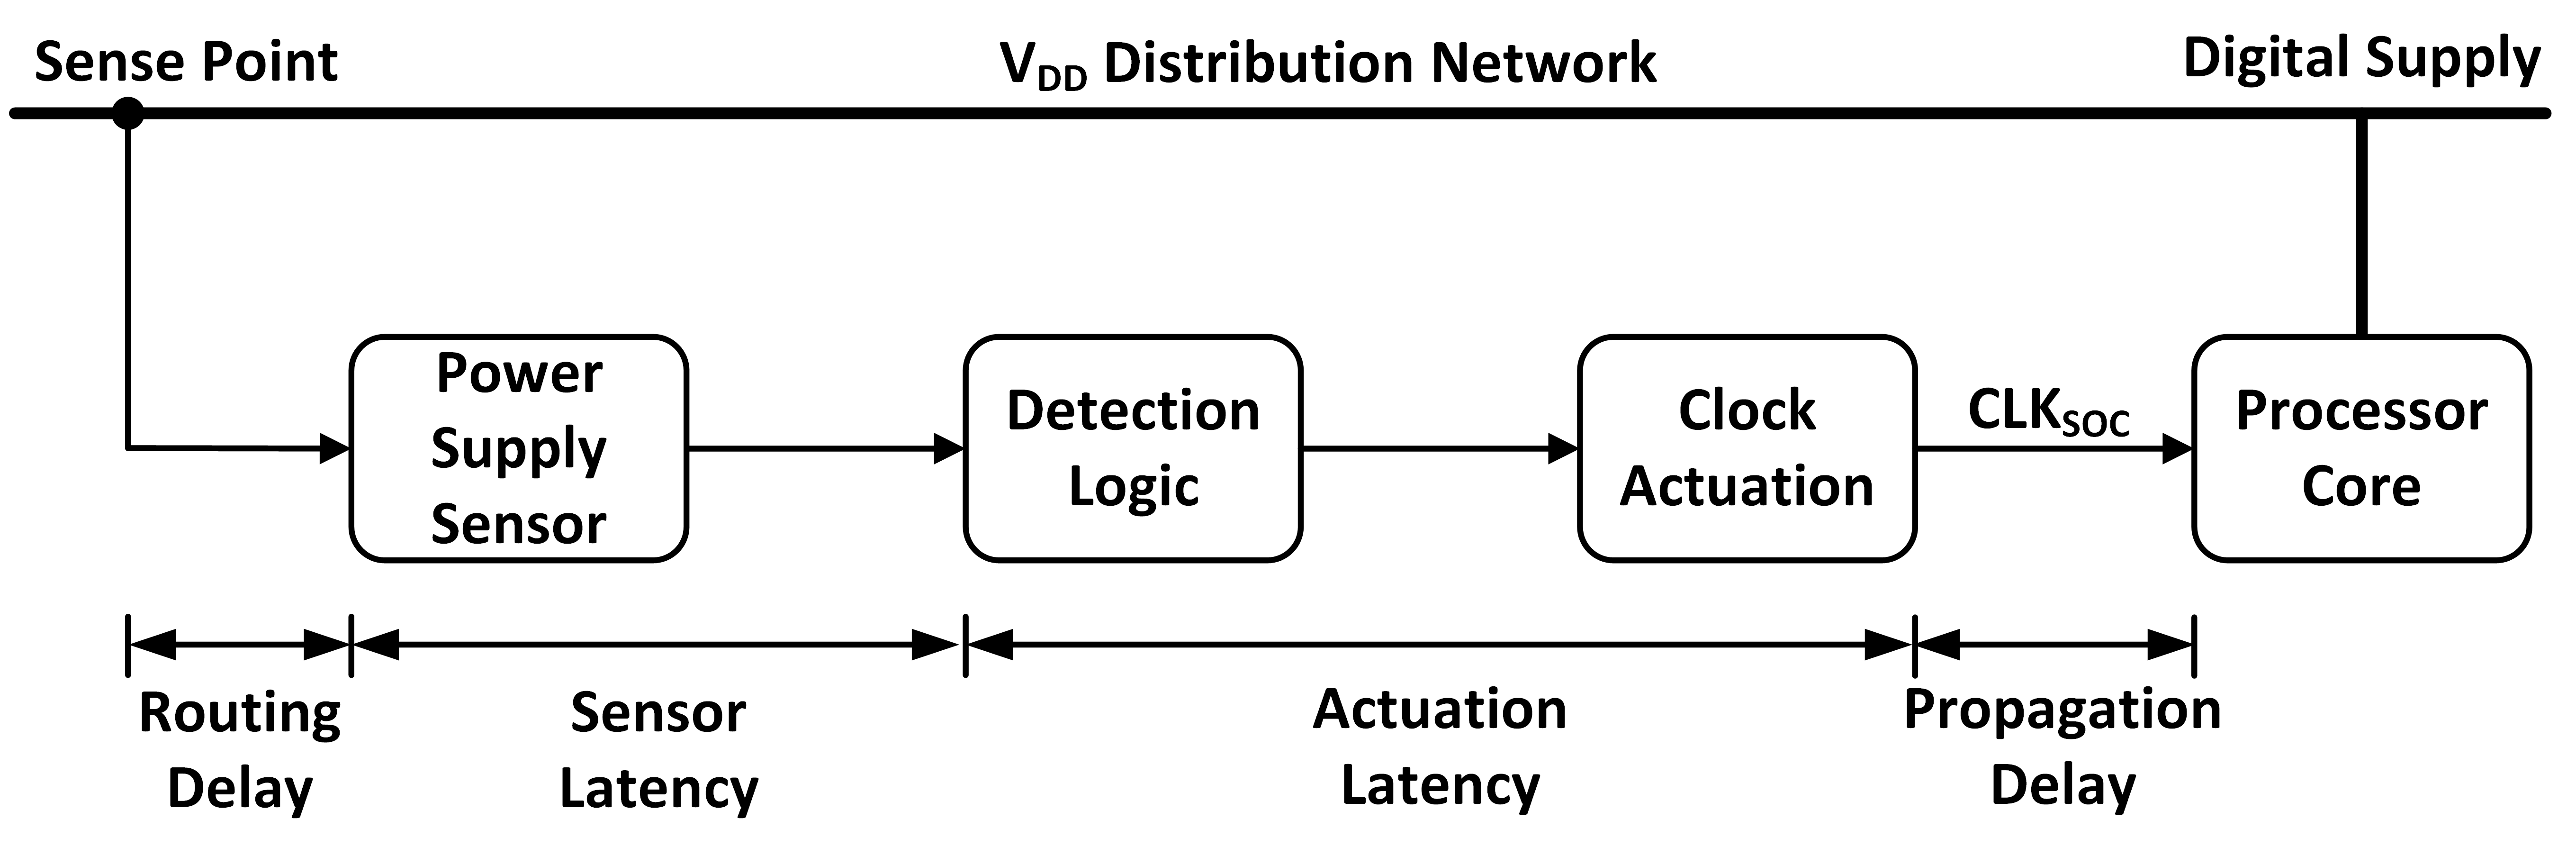
\includegraphics[width=\columnwidth]{fig_scope}
	\caption{Various latencies in adaptive clock system (adapted from \cite{hashimoto2018}).}
	\label{fig:scope}
\end{figure}

In comparing the PLL- and ACD-based adaptive clocking schemes, key metrics are identified: actuation latency, power/area, calibration, and frequency gain/$V_{MIN}$ reduction. Forecasts for these metrics in the predictive 7nm technology ASAP7 \cite{asap7} are also discussed.

\subsection{Actuation Latency}
\label{sec:ActuationLatency}
Minimizing actuation latency helps reduce overall system response time. In \cite{hashimoto2018}, the PLL-based actuation latency varies depending on the direction of $V_{DD}$ change due to the non-linear adaptation filter. As previously discussed, for decreases in $V_{DD}$, the latency is less than one clock cycle and limited by asynchronous propagation delay through the minimum function in Fig.\ \ref{fig:overview_pll} and the control bandwidth of the oscillator. The control port time constant is approximately $\frac{T_{VCO}}{2N}$ for the reported oscillator \cite{hashimoto2018}. Assuming the routing parasitic from the minimum logic to the oscillator control port is negligible, this allows a latency below one clock cycle at the reported $f_{MAX}$ = 5GHz, i.e. $t_{act} <$ 200ps.

Conversely, the ACD-based actuation latency is reported as 2 clock cycles at 3.4 GHz \cite{wilcox2015}, implying $t_{act} =$ 588ps. This is due to synchronizing $DroopDetected$ to the PLL clock domain  and generating the corresponding phase rotation enable signal as was shown in Fig.\ \ref{fig:detail_acd}.

We predict these results will be comparable in ASAP7. The actuation latency in \cite{wilcox2015} will remain 2 clock cycles by design. That in \cite{hashimoto2018} will remain less than one cycle again by design, with the potential for $t_{act}$ to be reduced due to increased $f_{T}$. One drawback may be higher resistance routing which could decrease oscillator control bandwidth if not carefully designed.

\subsection{Power/Area}
\label{sec:power_area}
While neither works report measured power and area overhead of the actuation or overall adaptation circuits, the use of a DLL in \cite{wilcox2015} is estimated to cost more. Consider phase mismatch and jitter amplification in the DLL \cite{wilcox2015}. The 40-phase DLL consists of 20 pseudo-differential delay cells, each designed as a pair of cross-coupled inverters with tunable MOS capacitor (MOSCAP) loads. In theory, the $k^{th}$ and $(k+20)^{th}$ phases have a standard deviation of $\sqrt{k} \sigma_{u}$ where $\sigma_{u}$ is one stage's delay variation. The DLL must, at a minimum, ensure phase monotonicity to guarantee glitchless phase rotations. $\sigma_{u}$ is directly correlates to $V_{t}$ and thereby area.

The DLL can also have power implications on the upstream PLL through system jitter specifications. Assume the DLL nears a 2$\times$ tuning range, similar of ring-based PLLs. Each DLL stage must achieve a min/max delay spread of 2$\times$. Fig.\ \ref{fig:dllasap7} shows schematic simulations in ASAP7 of an example delay stage operating at maximum $f_{CLK}=$ 3GHz. To achieve higher delay spread per stage, higher MOSCAP sizing is needed. However, this also decreases the RC bandwidth at each stage, increasing deterministic jitter amplification such as duty-cycle distortion (DCD) as also shown in Fig.\ \ref{fig:dllasap7}. To ensure jitter is not amplified through the DLL, the overall delay chain should target jitter amplification $<$ 1. Otherwise, power must be expended in the upstream PLL to reduce input jitter and DCD.
\vspace{-10pt}
\begin{figure}[h]
	\centering
	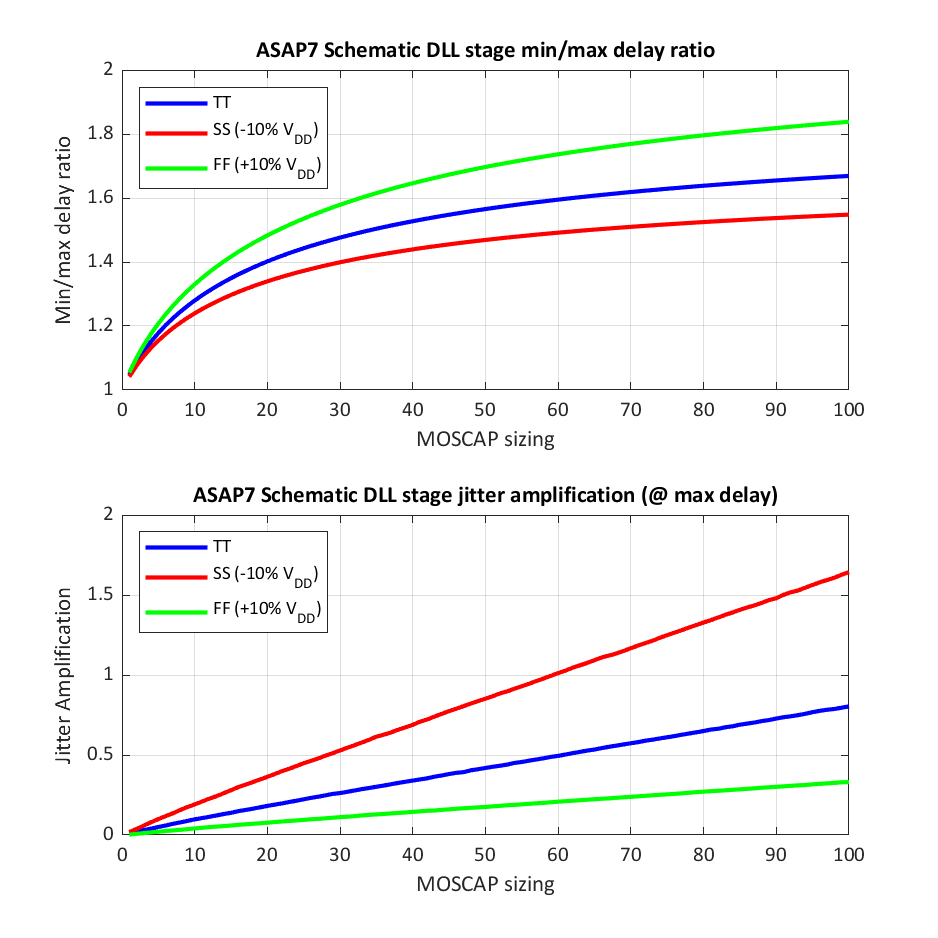
\includegraphics[width=0.8\columnwidth]{fig_dllasap7}
	%\caption{Schematic simulation of example DLL stage in ASAP7: min/max delay ratio (top) and jitter amplification (bottom) per stage.}
	\caption{Schematic simulation of example DLL stage in ASAP7.}
	\label{fig:dllasap7}
\end{figure}
\vspace{-15pt}
\subsection{Design \& Calibration}
\label{sec:calibrationoverhead}
Design-time complexity of the PLL-based scheme in \cite{hashimoto2018} involves an unconventional PLL loop, a detection filter overriding the VCO control and the restoring of PLL lock during frequency recovery by ramping the feedback divider value. Conversely, the ACD-based scheme in \cite{wilcox2015} is a simpler design that does not require modifications to a PLL, and instead inserts a phase rotator in the clock network between it and the SoC. Both works report manually calibrate supply sensor thresholds to optimize measured $f_{MAX}$ or $V_{MIN}$ margin \cite{hashimoto2018,wilcox2015}. The DLL in \cite{wilcox2015} incurs a further calibration overhead: the DLL can take up to 180 PLL clock cycles to frequency lock after start-up or during a dynamic voltage and frequency scaling (DVFS) event. To mitigate impact of supply noise, the CPU activity is limited during this time. In contrast, the PLL-based approach in \cite{hashimoto2018} does not incur calibration overhead beyond normal PLL locking, the dynamics of which can be particularly fine-tuned in a digital PLL. However, to restore clock frequency after a droop event, the non-linear filter in \cite{hashimoto2018} slowly adjusts the feedback divider (once every 32 reference clock cycles) to mitigate frequency overshoot and current surges during recovery.

\subsection{Silicon Performance}
\label{sec:performance}
The key performance metric reported in both adaptation schemes is reducing voltage/frequency margin. As \cite{hashimoto2018} claims, this is directly proportional to adaptation latency: the shorter the adaptation response time, the closer the SoC can operate to safety limits. Both systems achieve similar results. In terms of $V_{MIN}$, the PLL-based scheme achieves 5\% reduction at 4.65GHz \cite{hashimoto2018} while the ACD-based scheme reports up to 6\% reduction \cite{wilcox2015} at 4GHz. The PLL-based scheme also reports a 7.5\% gain in $f_{MAX}$ to 5GHz if $V_{DD}$ is unchanged \cite{hashimoto2018}. These results require integration of the adaptation system with the complete entire SoC, which may not be feasible in ASAP7 for this project scope: adaptation latency will be used as a proxy.

\subsection{Proposed Project Objectives}
\label{sec:proposal}
While reported in planar technologies \cite{hashimoto2018, wilcox2015}, the reduced actuation latency and the lack of immediate power, area, and calibration overhead for similar reported reduction in $V_{MIN}$ suggest the PLL-based adaptation circuit \cite{hashimoto2018} will be the favourable candidate in FinFET technologies. We propose to evaluate this in ASAP7 with the following project objectives:

\begin{enumerate}[(a)]
\item Initial design and power/area/latency estimates of the ACD-based actuator in \cite{wilcox2015}, in particular the DLL-based phase rotator. Estimated mismatch models may be required if not immediately available in ASAP7 \cite{asap7}.
\item Initial design and power/area/latency estimates of the PLL-based actuator in \cite{hashimoto2018}, in particular the PLL loop and non-linear filter interaction. Estimated models of the oscillator may be required.
\item (\textit{Time-permitting}) Investigations into possible improvements in \cite{hashimoto2018}, such as derivative loop filter control or modifications to non-linear filter to reduce frequency recovery time.
\end{enumerate}

\section{Conclusion}
\label{sec:conclusion}

This work compares the costs and effectiveness of ACD- and PLL-based adaptive clocking systems \cite{hashimoto2018,wilcox2015}. ACD-based systems exchange design complexity for higher power and area, but both systems achieve less than 2 cycle actuation latency and $V_{MIN}$ reductions by up to 6\%. The PLL-based system is predicted to achieve lower actuation latency and power/area in predictive 7nm CMOS, and initial designs of these systems are planned to evaluate this claim.


\bibliographystyle{IEEEtran}
\begingroup
\raggedright
\bibliography{references}
\endgroup

\end{document}
